\documentclass[14pt,a4paper]{extarticle}
\usepackage{graphicx}
\usepackage{caption} 
\usepackage{hyperref}
\usepackage[T1]{fontenc}
\usepackage[utf8x]{inputenc}
\usepackage{pdfpages}
\usepackage{libertine}
\usepackage{listings}
\usepackage{xcolor}
\usepackage{enumitem}
\renewcommand{\thesection}{\arabic{section}}
\renewcommand{\familydefault}{\sfdefault}

\definecolor{stringgreen}{rgb}{0.0, 0.5, 0.0}

\lstset{
  literate={ö}{{\"o}}1
           {ä}{{\"a}}1
           {ü}{{\"u}}1
           {Ö}{{\"O}}1
}

\lstdefinestyle{fish}{
	basicstyle=\small\ttfamily\color{black},
    keywordstyle=\color{blue},
	stringstyle=\medium\ttfamily\color{green},
    numberstyle=\tiny\color{gray},
    showstringspaces=false,
    tabsize=4,
	frame=single,
    breaklines=true,
    morekeywords={sudo,if,then,else,elif,fi,for,do,done,while,until,in},
}

\lstdefinestyle{json}{
	basicstyle=\small\ttfamily\color{black},
    showstringspaces=false,
    tabsize=2,
    breaklines=true,
}

\lstdefinestyle{sql}{
	basicstyle=\small\ttfamily\color{black},
    keywordstyle=\color{blue},
	stringstyle=\color{stringgreen},
    numberstyle=\tiny\color{gray},
    showstringspaces=false,
	frame=single,
    tabsize=4,
    breaklines=true,
	language=SQL
}

\colorlet{punct}{red!60!black}
\definecolor{delim}{RGB}{20,105,176}
\colorlet{numb}{magenta!60!black}

\hypersetup{
    colorlinks=true,
    linkcolor=blue,
    filecolor=blue,      
    urlcolor=blue,
    pdfborder={0 0 0},
    linktocpage      
}

\begin{document}
	\begin{titlepage}
		\centering
		{\scshape\LARGE Big Data \par}
		\vspace{2.5cm}
		{\huge\bfseries Graph Databases}
		\vfill
		{\normalsize von\par}
		{\normalsize Benjamin Ellmer (\textsc{S2210455012}) \par}
		\vspace{1cm}
		
\includegraphics[width=0.3\textheight]{images/logo.pdf} \par
		\vspace{1cm}
		{\large Mobile Computing Master \par}
		{\large FH Hagenberg \par}
		\vfill
		{\large \today\par}
	\end{titlepage}

	\section*{Installation}
	\noindent \textbf{Start Neo4j}
	\begin{lstlisting}[style=fish]
git clone https://github.com/Digital-Media/neo4j.git
docker compose -f neo4j/docker-compose.yml up -d
	\end{lstlisting}

	\noindent \textbf{Start Postgres}
	\begin{lstlisting}[style=fish]
docker run --name postgres-big-data-ex4 -e POSTGRES_PASSWORD=geheim -d postgres:14
	\end{lstlisting}

	\section*{Step 1 - Translation}
	\noindent \textbf{Drop, create and select schema:}
	\begin{lstlisting}[style=sql]
DROP SCHEMA IF EXISTS graph_demos CASCADE;
CREATE SCHEMA IF NOT EXISTS graph_demos;
SET search_path TO graph_demos;
	\end{lstlisting}

	\noindent \textbf{Create folks table:}
	\begin{lstlisting}[style=sql]
CREATE TABLE IF NOT EXISTS folks (
	id bigint NOT NULL,
	name varchar(100) NOT NULL,
	father bigint NULL,
	mother bigint NULL,
	PRIMARY KEY (id),
	CONSTRAINT father_fk FOREIGN KEY (father) REFERENCES folks(id),
	CONSTRAINT mother_fk FOREIGN KEY (mother) REFERENCES folks(id)
);
	\end{lstlisting}

	\noindent \textbf{Insert folks:}
	\begin{lstlisting}[style=sql]
INSERT INTO folks (id, name, father, mother) VALUES
(100, 'Alex', 20, 30),
(20, 'Dad', 10, null),
(30, 'Mom', null, null),
(10, 'Grandpa Bill', null, null),
(98, 'Sister Amy', 20, 30);
	\end{lstlisting}

	\noindent \textbf{Create vertices table:}
	\begin{lstlisting}[style=sql]
CREATE TABLE vertices (
	vertex_id bigint NOT NULL,
	alias varchar (255),
	label varchar (255),
	name varchar (255),
	type varchar (255),
	properties jsonb,
	PRIMARY KEY (vertex_id)
);
	\end{lstlisting}

	\noindent \textbf{Insert vertices:}
	\begin{lstlisting}[style=sql]
INSERT INTO vertices (vertex_id, alias, label, name, type) VALUES
(1, 'NAmerica', 'Location', 'North America', 'continent'),
(2, 'Europe', 'Location', 'Europe', 'continent'),
(3, 'USA', 'Location', 'United States', 'country'),
(4, 'UK', 'Location', 'United Kingdom', 'country'),
(5, 'England', 'Location', 'England', 'country'),
(6, 'Austria', 'Location', 'Österreich', 'country'),
(7, 'Idaho', 'Location', 'Idaho', 'state'),
(8, 'London', 'Location', 'London', 'city'),
(9, 'UpperAustria', 'Location', 'Oberösterreich', 'Bundesland'),
(10, 'Waldviertel', 'Location', 'Waldviertel', 'Viertel'),
(11, 'Grein', 'Location', 'Grein', 'city'),
(12, 'Andrea', 'Person', 'Andrea', 'person'),
(13, 'Bert', 'Person', 'Bert', 'person'),
(14, 'Christian', 'Person', 'Christian', 'person');
	\end{lstlisting}

	\newpage

	\noindent \textbf{Create edges table:}
	\begin{lstlisting}[style=sql]
CREATE TABLE edges (
	edge_id bigint NOT NULL,
	tail_vertex bigint REFERENCES vertices (vertex_id),
	head_vertex bigint REFERENCES vertices (vertex_id),
	label varchar(255),
	properties jsonb,
	PRIMARY KEY (edge_id),
	CONSTRAINT tail_vertex_fk FOREIGN KEY (tail_vertex) REFERENCES vertices(vertex_id),
	CONSTRAINT head_vertex_fk FOREIGN KEY (head_vertex) REFERENCES vertices(vertex_id)
);
	\end{lstlisting}

	\noindent \textbf{Insert edges:}
	\begin{lstlisting}[style=sql]
INSERT INTO edges (edge_id, tail_vertex, head_vertex, label) VALUES
(1, 3, 1, 'within'),
(2, 4, 2, 'within'),
(3, 5, 4, 'within'),
(4, 6, 2, 'within'),
(5, 7, 3, 'within'),
(6, 8, 5, 'within'),
(7, 9, 6, 'within'),
(8, 10, 9, 'within'),
(9, 11, 10, 'within'),
(10, 12, 7, 'born_in'),
(11, 12, 8, 'lives_in'),
(12, 13, 11, 'born_in'),
(13, 13, 8, 'lives_in'),
(14, 14, 8, 'born_in'),
(15, 12, 13, 'married'),
(16, 13, 12, 'married');
	\end{lstlisting}

	%\noindent \textbf{Create API Key} \\
	%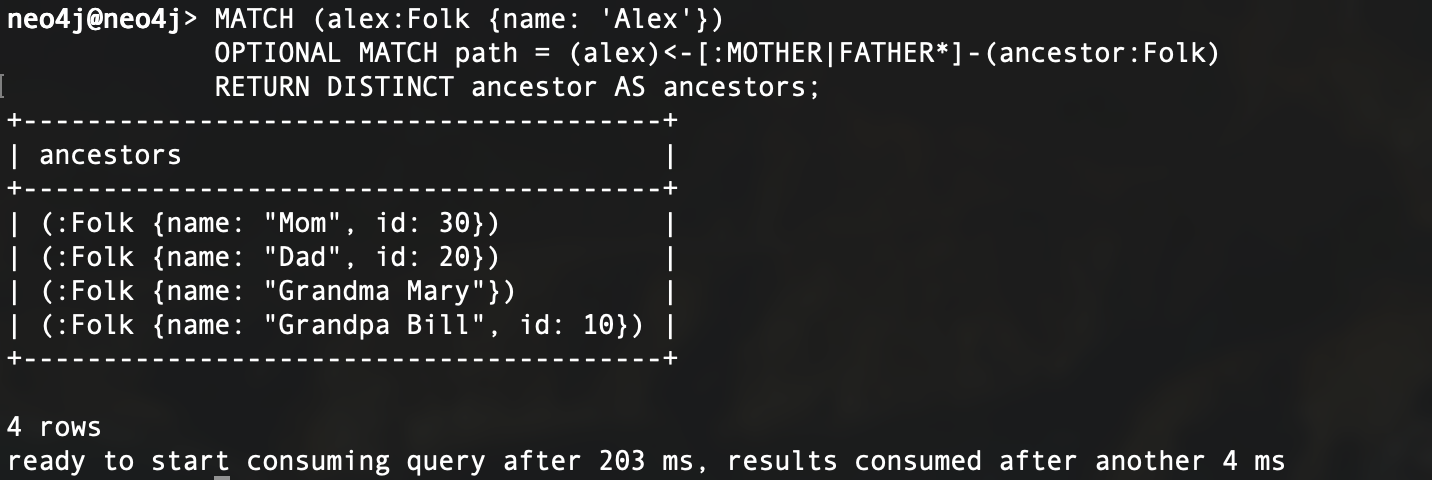
\includegraphics[width=\textwidth]{images/sc04.png}

	%\noindent \textbf{The pipeline fails because data is already in use} \\
	%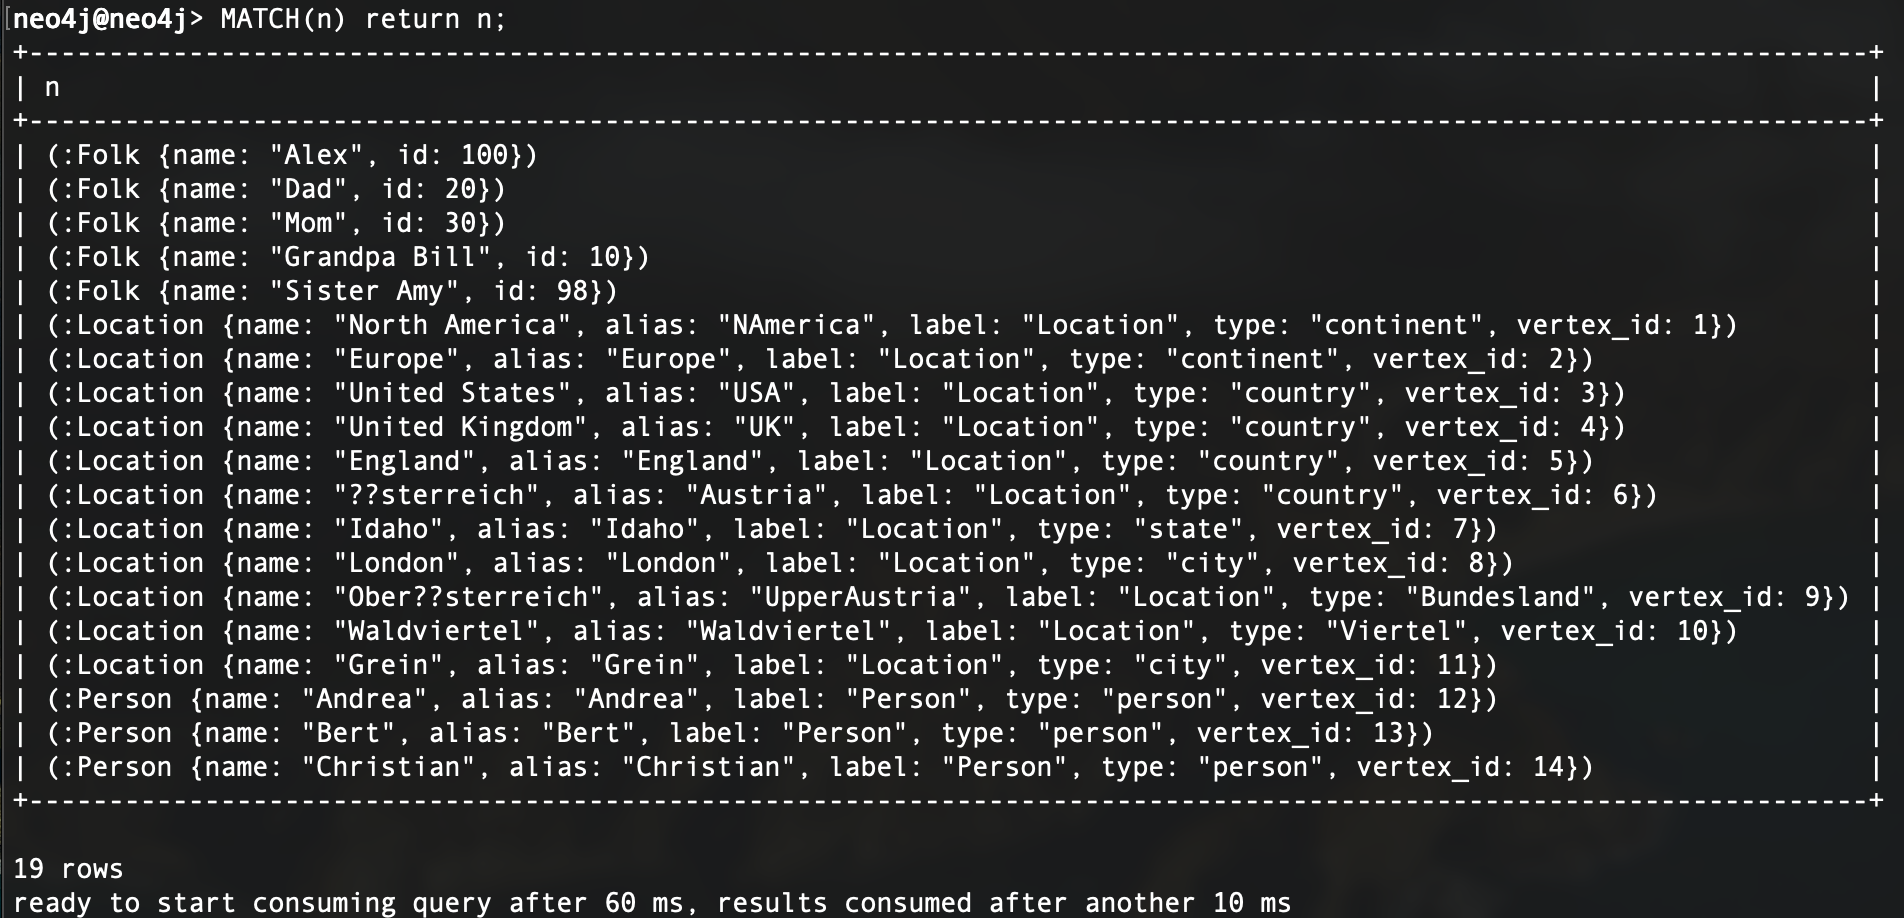
\includegraphics[width=\textwidth]{images/sc01.png} 
	%See \hyperref[listings:pipeline]{pipeline.conf} in appendix for the pipeline 
	%\begin{enumerate}[noitemsep]
		%\item Import the json file using mongoimport
	%\end{enumerate}

	%\newpage
	
	%\section*{Appendix}

	%\subsection*{.env}
	%\label{listings:envs}
	%\lstinputlisting[style=json]{.env}

\end{document}

